\documentclass[12pt]{article}
\usepackage[pdfborder={0 0 0.5 [3 2]}]{hyperref}%
\usepackage[left=1in,right=1in,top=1in,bottom=1in]{geometry}%
\usepackage[shortalphabetic]{amsrefs}%
\usepackage{amsmath}
\usepackage{enumerate}
% \usepackage{enumitem}
\usepackage{amssymb}                
\usepackage{amsmath}                
\usepackage{amsfonts}
\usepackage{amsthm}
\usepackage{bbm}
\usepackage[table,xcdraw]{xcolor}
\usepackage{tikz}
\usepackage{float}
\usepackage{booktabs}
\usepackage{svg}
\usepackage{mathtools}
\usepackage{cool}
\usepackage{url}
\usepackage{graphicx,epsfig}
\usepackage{makecell}
\usepackage{array}

\def\noi{\noindent}
\def\T{{\mathbb T}}
\def\R{{\mathbb R}}
\def\N{{\mathbb N}}
\def\C{{\mathbb C}}
\def\Z{{\mathbb Z}}
\def\P{{\mathbb P}}
\def\E{{\mathbb E}}
\def\Q{\mathbb{Q}}
\def\ind{{\mathbb I}}

\DeclareMathOperator{\spn}{span}
\DeclareMathOperator{\ran}{range}

\graphicspath{ {periodic/} }

\newtheorem{lemma}{Lemma}
\newtheorem{theorem}{Theorem}
\newtheorem{corollary}{Corollary}
\newtheorem{definition}{Definition}
\newtheorem{assumption}{Assumption}
\newtheorem{hypothesis}{Hypothesis}

\newtheorem{notation}{Notation}

\begin{document}

\section{Rough idea for 2-periodic pulse}

This is a rough sketch only, to see if this will work. Take a standard periodic 2-pulse, $2X_0$ is ``pulse distance'', $2X_1$ is ``period distance''.

\begin{enumerate}

\item Since system is Hamiltonian, we only have one equation we need to solve (SanStrut (3.9) and discussion on p. 2093).

\begin{align}\label{jumpeq}
\langle \Psi(-X_0), Q(X_0) \rangle - \langle \Psi(-X_1), Q(X_1) \rangle + R_0 &= 0
\end{align}

where $R_0 = \mathcal{O}(e^{-3 \alpha X_m})$, $X_m = \min\{X_i\}$.

\item This is a single equation with two unknowns, so we expect to have a family of solutions paramaterized by one of the unknowns. We can pick either one to be the paramater, but it makes sense to let $X_1$ be the parameter, since the idea is that all periods should be possible. The only possible restriction is that $X_1$ might have to be sufficiently large, but we will deal with that when it comes up. Thus the term $\langle \Psi(-X_1), Q(X_1) \rangle$ will be constant.

\item From Lemma 6.1 in San98, we have an expression for $\langle \Psi(-x), Q(x) \rangle$ for sufficiently large $x$.

\begin{equation}\label{alphabeta}
\langle \Psi(-x), Q(x) \rangle
= s_0 e^{-2 \alpha x} \sin(2 \beta x + \phi) + \mathcal{O}(e^{-(2 \alpha + \gamma) x})
\end{equation}

where $0 < \gamma \leq 1$.

\item Plug \eqref{alphabeta} into \eqref{jumpeq} to get

\begin{align}\label{jumpeq1}
s_0 e^{-2 \alpha X_0} \sin(2 \beta X_0 + \phi) - s_0 e^{-2 \alpha X_1} \sin(2 \beta X_1 + \phi) + \mathcal{O}(e^{-(2 \alpha + \gamma) X_m}) &= 0
\end{align}

The remainder term $R_0$ is incorporated into $\mathcal{O}(e^{-(2 \alpha + \gamma) X_m})$ term, since $R_0$ is equal or higher order.

\item Define the set

\begin{equation}\label{setR}
\mathcal{R} = \left\{ \exp\left(-\frac{\pi \alpha}{\beta}m\right) : m \in \N_0 \right\} \cup \{ 0 \}
\end{equation}

Since $\mathcal{R}$ is closed and bounded, is is compact, thus complete.

\item Define the following things

\begin{align*}
r_m &= e^{-(\pi \alpha /\beta) m} \in \mathcal{R} && m \in \N \\
a_i &= e^{-2\alpha X_i}e^{-\alpha \phi / \beta}\frac{1}{r_m}
\end{align*}

Note that

\begin{align*}
e^{-2 \alpha X_i} &= a_i r_m e^{\alpha \phi / \beta} \\
2 \beta X_i &= -(\beta / \alpha)\log a_i r_m - \phi 
\end{align*}

\item Substitute these into the LHS of \eqref{jumpeq1} to get 

\begin{align}\label{jumpeq2}
s_0 e^{\alpha \phi / \beta } a_0 r_m \sin \left( - \frac{\beta}{\alpha} \log (a_0 r_m) \right) - s_0 e^{\alpha \phi / \beta } a_1 r_m \sin \left( - \frac{\beta}{\alpha} \log (a_1 r_m) \right) + \mathcal{O}(r_m^{1 + \gamma / 2 \alpha}) &= 0 \\
\end{align}

where we have chosen the $X_i$ sufficiently large so that $e^{-2 \alpha X_i} < r_m$ for all $i$. Divide both sides by $r_m$ and the constant $s_0 e^{\alpha \phi / \beta }$ to get

\begin{align}\label{jumpeq3}
a_0 \sin \left( - \frac{\beta}{\alpha} \log (a_0 r_m) \right) - a_1 \sin \left( - \frac{\beta}{\alpha} \log (a_1 r_m) \right) + \mathcal{O}(r_m^{\gamma / 2 \alpha}) &= 0 \\
\end{align}

By the clever choice of $r_m$, as in SanStrut, the $r_m$ term inside the sine terms die, leaving us with

\begin{align}\label{jumpeq4}
a_0 \sin \left( - \frac{\beta}{\alpha} \log a_0 \right) - a_1 \sin \left( - \frac{\beta}{\alpha} \log a_1 \right) + \mathcal{O}(r_m^{\gamma / 2 \alpha}) &= 0 \\
\end{align}

Note that $r_m$ now only occurs in the remainder term, which is what we wanted.

\item We want to use the IFT to solve for $a_0$ in terms of $r_m$, with $a_1$ as a parameter. Thus we want to solve

\begin{align*}
G(a_0, r_m; a_1) = 
a_0 \sin \left( - \frac{\beta}{\alpha} \log a_0 \right) - a_1 \sin \left( - \frac{\beta}{\alpha} \log a_1 \right) + \mathcal{O}(r_m^{\gamma / 2 \alpha}) &= 0
\end{align*}

\item To use the IFT, we need to find values of $a_0$ and $r_m$ so that $G(a_0, r_m; a_1) = 0$. To make things easier, we first take $r = 0$ (which we can do by how we defined $\mathcal{R}$ to get rid of the remainder term, leaving us with

\begin{align*}
G(a_0, 0; a_1) = 
a_0 \sin \left( - \frac{\beta}{\alpha} \log a_0 \right) - a_1 \sin \left( - \frac{\beta}{\alpha} \log a_1 \right)
\end{align*}

With $r_m$ out of the picture, define

\begin{equation}
f(a_0, a_1) = 
a_0 \sin \left( - \frac{\beta}{\alpha} \log a_0 \right) - a_1 \sin \left( - \frac{\beta}{\alpha} \log a_1 \right)
\end{equation}

We note the following.

\begin{enumerate}
	\item $f(a_1, a_0) = -f(a_0, a_1)$, i.e. $f$ is antisymmetric with respect to its two arguments.

	\item $f(a_0, a_0) = 0$. In this case, we have

	\begin{align*}
	G(a_0, r_m; a_0) = \mathcal{O}(r_m^{\gamma / 2 \alpha})
	\end{align*}

	so the lengths $X_i$ (which are the same) drop out of the equation. By the Hamiltonian nature and some handwaving, this has to be satisfied (otherwise there is a jump in the energy). So in this case, we have a periodic wavetrain.

	\item $f(0, 1) = f(1, 0) = 0$. This uses what we know about the limit of the sine term when we approach 0.
\end{enumerate}

We are looking for the zero set of $f(a_0, a_1)$. We know that this zero set contains $a_0 = a_1$, which corresponds to the periodic wavetrain. We also know it contains $(0, 1)$ and $(1, 0)$. By (anti-)symmetry, we only need consider what happens when $a_1 \leq a_0$.\\

Mathematica plotting suggests that a pitchfork bifurcation takes place, and along the branch we will have a periodic double pulse. This bifurcation must take place along the $a_0 = a_1$ line where $f_{a_0}(a_0, a_0) = 0$. (Otherwise we could apply the IFT, and we know that has to give us the line $a_0 = a_1$). Taking this derivative, we get

\begin{align*}
f_{a_0}(a_0, a_0) &= 
\sin \left( - \frac{\beta}{\alpha} \log a_0 \right)
+ a_0 \cos \left( - \frac{\beta}{\alpha} \log a_0 \right)- \frac{\beta}{\alpha} \frac{1}{a_0} \\
&= \sin \left( - \frac{\beta}{\alpha} \log a_0 \right) - \frac{\beta}{\alpha} \cos \left( - \frac{\beta}{\alpha} \log a_0 \right)
\end{align*}

This derivative is 0 when

\begin{align*}
\tan \left( -\frac{\beta}{\alpha} \log a_0 \right) &=  \frac{\beta}{\alpha} \\
-\frac{\beta}{\alpha} \log a_0 &= \arctan \left( \frac{\beta}{\alpha}\right) \\ 
a_0 &= \exp \left( -\frac{\alpha}{\beta} \arctan \left( \frac{\beta}{\alpha}\right) \right)
\end{align*}

\item Change coordinates so that we can get this (more or less) into the normal form of a pitchfork bifurcation. This is not hard to do, since there is always a zero along the diagonal. Let

\begin{align*}
x &= \frac{1}{2}(a_1 - a_0) \\
y &= \frac{1}{2}(a_1 + a_0)
\end{align*}

Inverting this, we have

\begin{align*}
a_0 &= y - x \\
a_1 &= y + x
\end{align*}

Substituting this into our expression for $f(a_0, a_1)$ yields

\begin{equation}\label{fxy}
f(x, y) = 
(y - x) \sin \left( - \frac{\beta}{\alpha} \log(y - x) \right) - (y + x) \sin \left( - \frac{\beta}{\alpha} \log (y + x) \right)
\end{equation}

It is easy to see from \eqref{fxy} that $f(-x, y) = -f(x, y)$. Thus in terms of the (yet to be proved) pitchfork normal form, the bifurcation parameter is $y$.\\

Using what we did above, we expect that a pitchfork bifurcation will take place at

\begin{equation}\label{pitchpt}
(x_0, y_0) = \left( 0, \exp \left( -\frac{\alpha}{\beta} \arctan \left( \frac{\beta}{\alpha}\right) \right) \right)
\end{equation}

To verify this, we need to check a bunch of derivatives. This is annoying, but not difficult. For the first derivatives, we have

\begin{align*}
f_x(x, y) &= -\sin \left( - \frac{\beta}{\alpha} \log(y - x) \right) - 
\sin \left( - \frac{\beta}{\alpha} \log(y + x) \right) \\
&+\frac{\beta}{\alpha} \cos \left( - \frac{\beta}z{\alpha} \log(y - x) \right) + \frac{\beta}{\alpha} \cos \left( - \frac{\beta}{\alpha} \log(y + x) \right) \\
f_y(x, y) &= \sin \left( - \frac{\beta}{\alpha} \log(y - x) \right) - 
\sin \left( - \frac{\beta}{\alpha} \log(y + x) \right) \\
&-\frac{\beta}{\alpha} \cos \left( - \frac{\beta}{\alpha} \log(y - x) \right) + \frac{\beta}{\alpha} \cos \left( - \frac{\beta}{\alpha} \log(y + x) \right)
\end{align*}

Plugging in $(x_0, y_0)$ from \eqref{pitchpt} and noting that

\begin{align*}
\sin \left( \arctan \left( \frac{\beta}{\alpha}\right) \right) &=
\frac{\beta}{\sqrt{\alpha^2 + \beta^2}} \\
\cos \left( \arctan \left( \frac{\beta}{\alpha}\right) \right) &=
\frac{\alpha}{\sqrt{\alpha^2 + \beta^2}} \\
\frac{\beta}{\alpha} \cos \left( \arctan \left( \frac{\beta}{\alpha}\right) \right) &=
\frac{\beta}{\sqrt{\alpha^2 + \beta^2}} \\
\end{align*}

it is easy to see that both $f_x(x_0, y_0) = 0$ and $f_y(x_0, y_0) = 0$. We now have to check the second derivatives. From Mathematica, we have

\begin{align*}
f_{xx}(x, y) &= -(y-x) \left(-\frac{\beta^2 \sin \left(\frac{\beta \log (y-x)}{\alpha}\right)}{\alpha^2 (y-x)^2}-\frac{\beta
   \cos \left(\frac{\beta \log (y-x)}{\alpha}\right)}{\alpha (y-x)^2}\right)\\
   &+(x+y) \left(-\frac{\beta^2
   \sin \left(\frac{\beta \log (x+y)}{\alpha}\right)}{\alpha^2 (x+y)^2}-\frac{\beta \cos \left(\frac{\beta
   \log (x+y)}{\alpha}\right)}{\alpha (x+y)^2}\right)\\
   &-\frac{2 \beta \cos \left(\frac{\beta \log
   (y-x)}{\alpha}\right)}{\alpha (y-x)}+\frac{2 \beta \cos \left(\frac{\beta \log (x+y)}{\alpha}\right)}{\alpha
   (x+y)}
\end{align*}

Mathematica tells us that $f_{xx}(x_0, y_0) = 0$. It also tells us that 
$f_{yy}(x_0, y_0) = 0$, although we don't need that for the pitchfork. The mixed derivative $f_{xy}$ is (again from Mathematica)

\begin{align*}
f_{xy}(x, y) &= -\frac{\beta^2 \sin \left(\frac{\beta \log (y-x)}{\alpha}\right)}{\alpha^2 (y-x)}-\frac{\beta^2 \sin
   \left(\frac{\beta \log (x+y)}{\alpha}\right)}{\alpha^2 (x+y)}+\frac{\beta \cos \left(\frac{\beta \log
   (y-x)}{\alpha}\right)}{\alpha (y-x)}+\frac{\beta \cos \left(\frac{\beta \log (x+y)}{\alpha}\right)}{\alpha (x+y)}
\end{align*}

Evaluating this at $(x_0, y_0)$ gives us

\begin{align*}
f_{xy}(x_0, y_0) &= \frac{2\beta}{\alpha\sqrt{\alpha^2 + \beta^2}} \left( \alpha + \frac{\beta^2}{\alpha} \right)\exp\left( \frac{\alpha}{\beta} \arctan \left( \frac{\beta}{\alpha}\right) \right) \\
&= \frac{2 \beta}{\alpha^2}\sqrt{ \alpha^2 + \beta^2 }
\exp\left( \frac{\alpha}{\beta} \arctan \left( \frac{\beta}{\alpha}\right) \right) \\
\end{align*}

Since $\alpha, \beta > 0$, $f_{xy}(x_0, y_0) > 0$. Let $k_1 = f_{xy}(x_0, y_0)$. Finally, we check the third derivative with respect to $x$. This is a mess, but from Mathematica we have

\begin{align*}
f_{xxx}(x_0, y_0)
&= -\frac{2 \beta}{\alpha^2}\sqrt{ \alpha^2 + \beta^2 }
\exp\left( \frac{2\alpha}{\beta} \arctan \left( \frac{\beta}{\alpha}\right) \right) < 0\\
\end{align*}

Let $k_2 = -f_{xxx}(x_0, y_0) > 0$. \\

We have verified that a pitchfork bifurcation occurs at $(0, y_0)$. In fact, near the bifurcation point $(0, y_0)$, we have the following Taylor expansion

\begin{align*}
f(x, y) = k_1 x (y - y_0) - \frac{k_2}{6} x^3 + \text{h.o.t.}
\end{align*}

Matlab plot suggests that the two arms of the pitchfork connect to the points $(x,y) = (\pm 1/2, 1/2)$, which correspond to $(a_0, a_1) = (1, 0)$ and $(a_0, a_1) = (0, 1)$. A plot of the arms of the pitchfork from the Taylor expansion together with the zeros of $f(x,y)$ (computed numerically) is given below.

\begin{figure}[H]
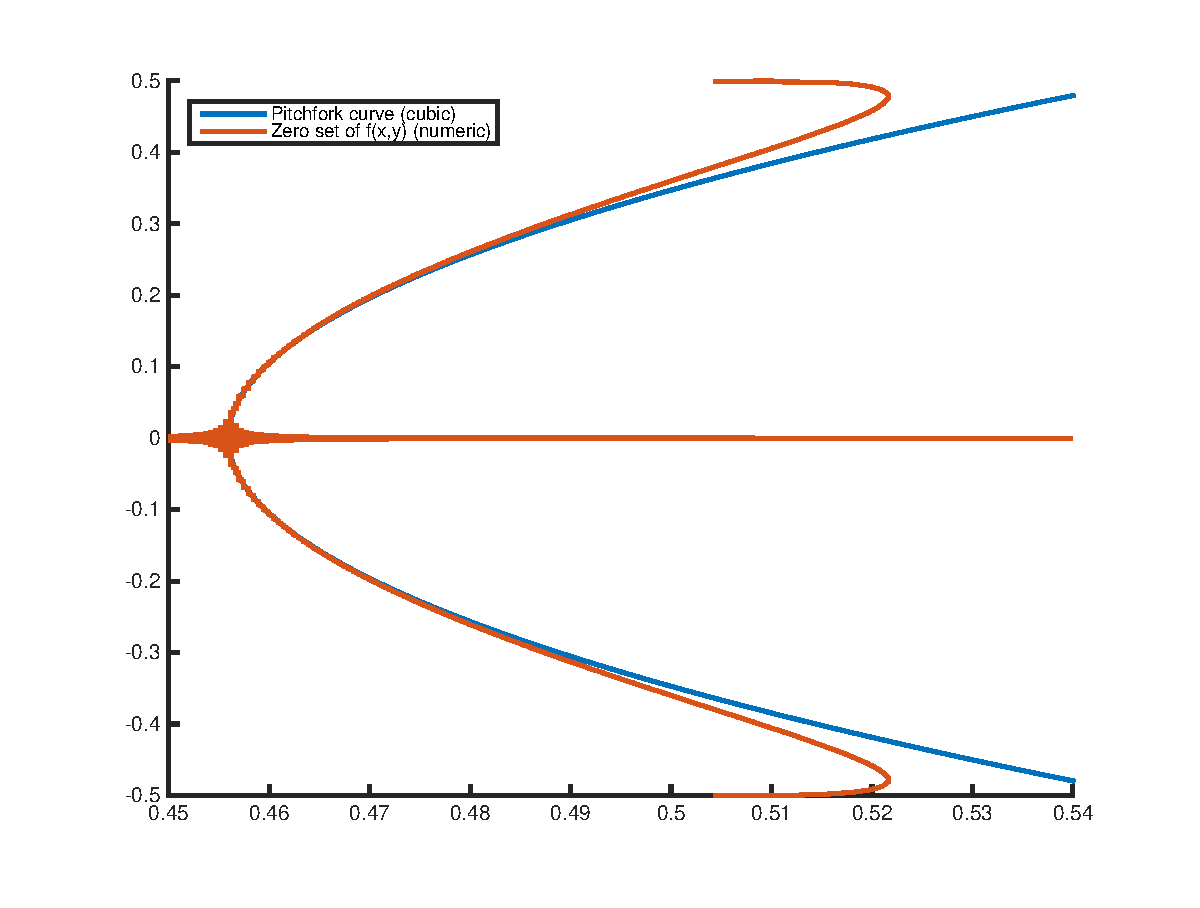
\includegraphics[width=10cm]{pitchfork.eps}
\end{figure}

Of course, I have no idea how to show this is actually true.

\item IGNORE THE REST OF THIS FOR NOW. THE IDEA IS RIGHT, BUT WE ARE TRYING TO GET THE REST OF THE BIFURCATION PICTURE.

\item To use the IFT, we need to check the derivative of $G$ with respect to $a_0$ at $(a_0, r) = (a_0^0(\delta(a_1)), 0)$. From SanStrut (3.13) and the longer writeup, this is 

\begin{align*}
\frac{\partial}{\partial a_0} &a_0 \sin \left( -\frac{\beta}{\alpha} \log a_0 \right)\Big|_{a_0 = a_0^0(\delta(a_1))} \\
&= \sin \left( - \frac{\beta}{\alpha} \log a_0 \right)\Big|_{a_0 = a_0^0(\delta(a_1))}  + a_0 \cos \left( - \frac{\beta}{\alpha} \log a_0 \right)\left( -\frac{\beta}{\alpha} \frac{1}{a_0} \right) \Big|_{a_0 = a_0^0(\delta(a_1))} \\
&= \sin \left( - \frac{\beta}{\alpha} \log a_0 \right) \Big|_{a_0 = a_0^0(\delta(a_1))}  -\frac{\beta}{\alpha} \cos \left( - \frac{\beta}{\alpha} \log a_0 \right) \Big|_{a_0 = a_0^0(\delta(a_1))} \\
&= \sin \left( \delta(a_1) \right) -\frac{\beta}{\alpha} \cos \left( \delta(a_1) \right) \\
&\approx -\frac{\beta}{\alpha}
\end{align*}

since for sufficiently small $a_1$, $\delta(a_1)$ is close to 0. Obviously, we will make this more precise. The whole point is that this is nonzero. Thus we can use the IFT to solve for $a_0$ in terms of $r$, i.e. we can find a smooth function $a_0(r)$ such that $a_0(0) = a_0^0(\delta(a_1)$ and near $(a_0, r) = (a_0^0(\delta(a_1)), 0)$ we have

\begin{align*}
\tilde{G}(a_0(r; a_1), r; a_1) = 0
\end{align*}

\item Let $r_0 > 0$ be sufficiently small so that the previous part works. Then chose any $m$ such that $r_m < r_0$. Then we have

\begin{align*}
G(a_0(r_m; a_1), r_m; a_1) = \tilde{G}(a_0(r_m; a_1), r_m; a_1) = 0
\end{align*}

\item Now we put things back in terms of the $X_i$, which is what we are about. Taking $r = r_m$, we can show that

\[
a_i = e^{(\pi \alpha / \beta) m} e^{-\alpha \phi / \beta}e^{-2 \alpha X_i}
\]

From what we did above and with much handwaving,\begin{align*}
\tilde{G}(a_0(r; a_1), r; a_1) = 0
\end{align*} we have $a_0 \approx 1$, in which case we have

\[
X_0 \approx \frac{\pi}{2 \beta} m + \frac{\phi}{2 \beta}
\]

What we did above works for any $a_1$ as long as it is sufficiently small, thus we can take any $X_1$ we want, as long as it is sufficiently large.

\end{enumerate}

\end{document}